\chapter{Projekt systemu}
\begin{figure}[ht]
	\begin{center}
		\resizebox{\textwidth}{!}{
			\begin{tikzpicture}[
					node distance=2.5cm, % Odstęp między węzłami
					align=center, % Wyśrodkowanie tekstu w węzłach
					>=latex, % Strzałki w stylu LaTeX
					%every node/.style={draw, text width=3cm} % Styl węzłów
				]

				\node[rectangle, minimum width=5cm, draw=black] (full_frame) {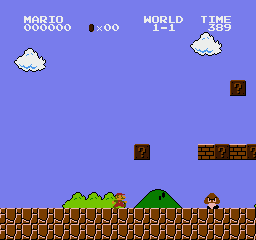
\includegraphics[width=4cm]{img/full_frame.png}\\Obraz generowany przez emulator NES};

				\node[right of=full_frame, xshift=6cm, draw=black] (compressed_frame) {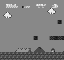
\includegraphics[width=2.5cm]{img/compressed_frame.png} \\Skompresowany obraz};
				\node (model) [right of=compressed_frame, draw = black, minimum height=2cm, xshift=2cm] {Model};
				\node (controller) [right of=model, draw=black, minimum height = 2cm, xshift=1cm, minimum width = 2cm] {Przyciski\\kontrolera\\NES};

				\draw[<-] (compressed_frame.west) -- (full_frame.east) node[midway] {Zmniejszenie\\ rozmiaru i \\ konwersja na skalę \\szarości};
				\draw[<-] (model.west) -- (compressed_frame.east) node[midway]{Konwersja\\na tensor};
				\draw[<-] (controller.west) -- (model.east) node[midway] {Predykcja\\wciśnięć};

			\end{tikzpicture}
		}
	\end{center}
	\caption{Ogólny schemat działania programu}
	\label{fig:sys_diagram}
\end{figure}
